\section{Quick reminder - What is the SpaceAPI?}

\begin{frame}[c]{What is the SpaceAPI}
    \begin{itemize}
        \item A JSON schema
        \item Describes your hackerspace
        \item Mostly static but may contain dynamic data
    \end{itemize}
\end{frame}

\begin{frame}[fragile]{SpaceAPI Excerpt}
    \begin{minted}[fontsize=\footnotesize]{json}
{
    "api": "0.13",
    "contact": {
        "email": "vorstand@lists.coredump.ch",
        "twitter": "@coredump_ch"
    },
    "sensors": {
        "people_now_present": [
            {
                "location": "Hackerspace",
                "value": 0
            }
        ]
    },
    "state": {
        "message": "Open Mondays from 20:00",
        "open": false
    }
}
    \end{minted}
\end{frame}

\section{The Beginning}

\begin{frame}[c]{Requirement}
    \begin{itemize}
        \item Serve SpaceAPI JSON data
        \item Mostly static except state and sensors
        \item Endpoint to update sensor data
    \end{itemize}
\end{frame}

\begin{frame}[c]{A 100 Line Python Script}
    \begin{itemize}
        \item Our first implementation was \~100 lines of Python\footnote{\url{https://github.com/coredump-ch/status/tree/1ae92a58c13b5ee106671092717f1bf4b4b9ee97}}
        \item Hacky but worked
    \end{itemize}
\end{frame}

\begin{frame}[c]{A 100 Line Python Script}
    \centering
    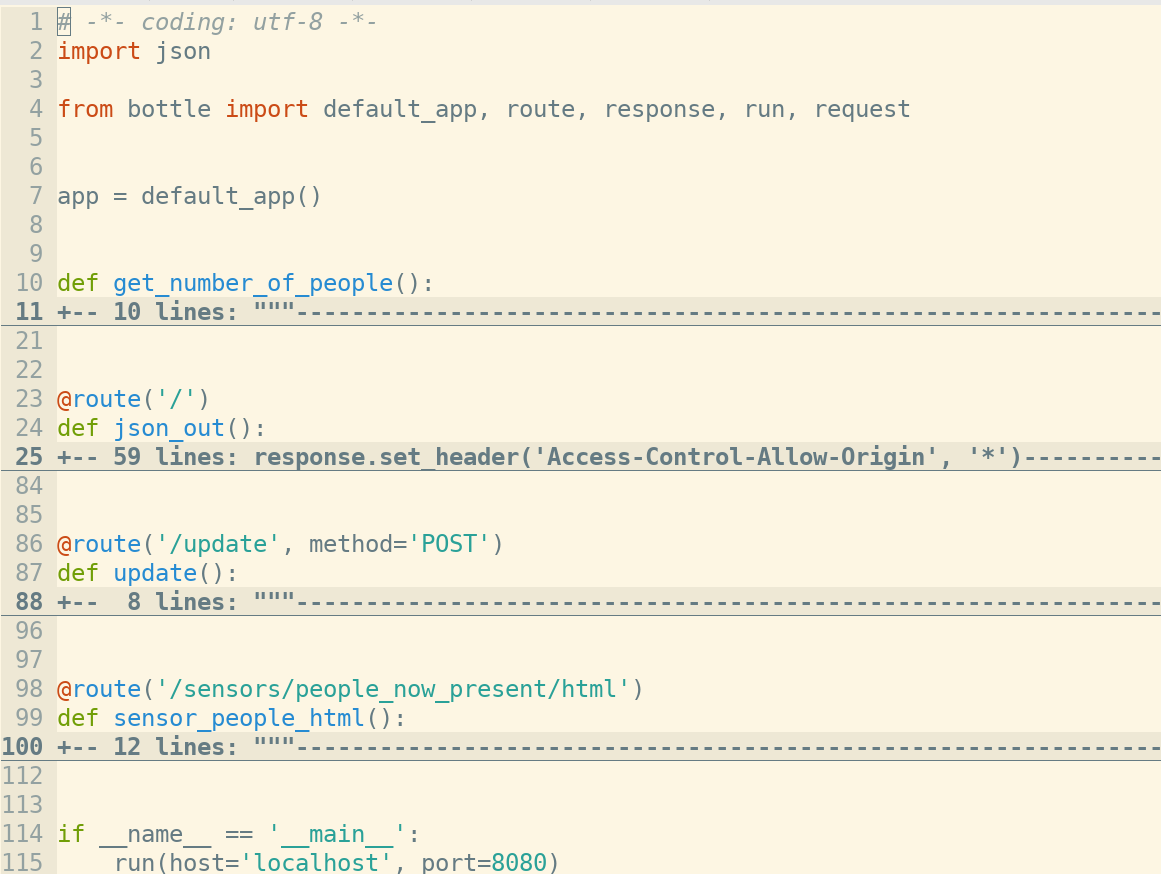
\includegraphics[height=0.98\textheight]{./spaceapi_in_rust/python2.png}
\end{frame}

\begin{frame}[fragile]{Reading the sensor...}
    \begin{minted}{python}
def get_number_of_people():
    """
    Return an integer or None.
    """
    people = None
    try:
        with open('people.txt', 'r') as f:
            people = int(f.read().strip())
    except:
        pass
    return people
    \end{minted}
\end{frame}

\begin{frame}[fragile]{Updating the sensor...}
    \begin{minted}{python}
@route('/update', method='POST')
def update():
    """
    Update the data in a text file.
    TODO: Public / Private key crypto.
    """
    people = int(request.POST.get('people'))
    with open('people.txt', 'w') as f:
        f.write(str(people))
    return 'OK'
    \end{minted}
\end{frame}

\begin{frame}[c]{Hacky, but actually worked!}
    \begin{itemize}
        \item Hacky but worked
        \item Probably a race conditions with the file access?
        \item Ugly to extend with further sensors
    \end{itemize}
\end{frame}

\section{Rewrite it in Rust!}

\begin{frame}[c]{Why?}
    \begin{itemize}
        \item If it worked why rewrite it?
        \pause\item Learn Rust
        \item Have a reasonable sized project
    \end{itemize}
\end{frame}

\begin{frame}[c]{Overengineer it!}
    \centering
    
\includegraphics[height=0.8\textheight]{./spaceapi_in_rust/overengineer_all_the_things.jpg}
\end{frame}

\begin{frame}[c]{Goals}
    \begin{itemize}
        \item Encode the SpaceAPI rules in the type system \\
            $\rightarrow$ Impossible to generate non conforming JSON
        \item Use a better backend for data storage
        \item Make it reusable for other hackerspaces
    \end{itemize}
\end{frame}

\begin{frame}[c]{Current Status}
    \begin{itemize}
        \item spaceapi-rs\footnote{\url{https://github.com/coredump-ch/spaceapi-rs}}
            \begin{itemize}
                \item SpaceAPI schema encoded in the type system
                \item Serialization / Deserialization
            \end{itemize}
        \item spaceapi-server-rs\footnote{\url{https://github.com/coredump-ch/spaceapi-server-rs}}
            \begin{itemize}
                \item Server implemented with Iron
                \item Reads sensor values from Redis DB
                \item Allows updating sensor values
            \end{itemize}
        \item status\footnote{\url{https://github.com/coredump-ch/status}}
            \begin{itemize}
                \item Implementation for coredump
            \end{itemize}
    \end{itemize}
\end{frame}

\subsection{spaceapi-rs}

\begin{frame}[fragile]{Data Types}
    \begin{minted}{rust}
pub struct Status {
    pub api: String,
    pub space: String,
    pub logo: String,
    pub url: String,
    pub location: Location,
    pub contact: Contact,
    ...
}
    \end{minted}
\end{frame}

\begin{frame}[c]{Difficulties}
    \begin{itemize}
        \item SpaceAPI specs don't allow null for optional entries
        \item \texttt{rustc\_serialize} serialized `Option<T>` to null \\
            \pause$\rightarrow$ We rolled our own serialization with an `Optional<T>` type
        \item Serde solved this quite elegant
    \end{itemize}
\end{frame}

\begin{frame}[fragile]{Serde}
    \begin{minted}{rust}
#[derive(Serialize, Deserialize, Default, Debug, Clone)]
pub struct Location {
    #[serde(skip_serializing_if = "Option::is_none")]
    pub address: Option<String>,
    pub lat: f64,
    pub lon: f64,
}
    \end{minted}
    \pause\begin{minted}{rust}
#[derive(Serialize, Deserialize, Debug, Clone, PartialEq)]
pub struct Sensors {
    #[serde(default, skip_serializing_if = "Vec::is_empty")]
    pub people_now_present: Vec<PeopleNowPresentSensor>,
    #[serde(default, skip_serializing_if = "Vec::is_empty")]
    pub temperature: Vec<TemperatureSensor>,
}
    \end{minted}
\end{frame}

\begin{frame}[fragile]{Find the problem}
    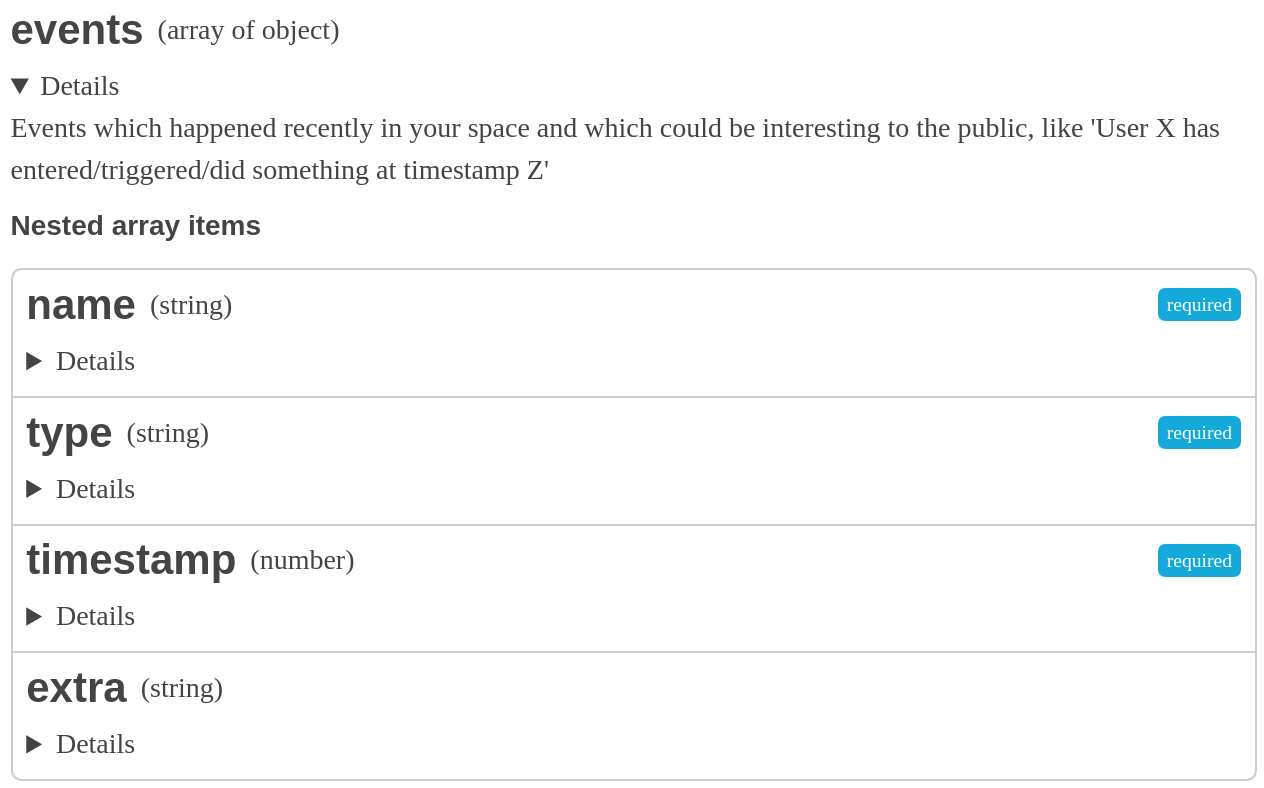
\includegraphics[height=0.98\textheight]{./spaceapi_in_rust/events.png}
\end{frame}

\begin{frame}[c,fragile]{Keywords\ldots}
    Rust doesn't like keywords as identifier\ldots
    \begin{minted}{shell}
error: expected identifier, found keyword `type`
  --> src/status.rs:52:9
   |
52 |     pub type: String,
   |         ^^^^
    \end{minted}
\end{frame}

\begin{frame}[c,fragile]{Serde to the rescue!}
    \begin{minted}{rust}
#[derive(Serialize, Deserialize, Default, Debug, Clone, PartialEq)]
pub struct Event {
    pub name: String,
    #[serde(rename = "type")]
    pub _type: String,
    pub timestamp: u64,
    #[serde(skip_serializing_if = "Option::is_none")]
    pub extra: Option<String>,
}
    \end{minted}
\end{frame}

